\documentclass[sigconf,authorversion,nonacm]{acmart}

\usepackage{minted}
\usemintedstyle{borland}
\setminted{linenos=true,fontsize=\large}

\usepackage{fontspec}
\setmonofont{Fira Code Retina}[Scale=MatchLowercase]

\captionsetup{justification=centering,margin=1cm}

\AtBeginDocument{%
  \providecommand\BibTeX{{%
    \normalfont B\kern-0.5em{\scshape i\kern-0.25em b}\kern-0.8em\TeX}}}

\begin{document}

\title{Tarea 6 \\ Lógica difusa}

\author{Mario Emilio Jiménez Vizcaíno}
\email{A01173359@itesm.mx}
\affiliation{}

\author{Jesus Abraham Haros Madrid}
\email{A01252642@itesm.mx}
\affiliation{}


\maketitle

\section{Descripción del problema}


\section{Descripción del sistema difuso}

\subsection{Funciones de membresía para las variables de entrada}

\subsection{Funciones de membrería para la variable de salida}

\subsection{Reglas}

\subsection{Forma de implicación}

\section{Resultados}
\subsection{Con coeficiente de fricción 0.1}
% \begin{figure}[H]
%   \centering
%   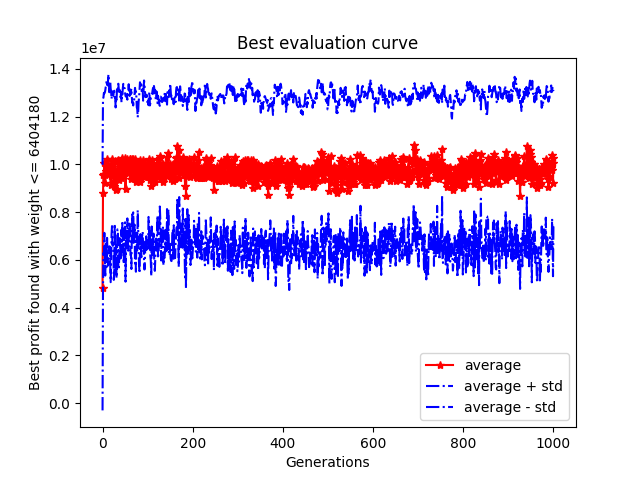
\includegraphics[width=210pt]{simple.png}
% \end{figure}

\subsection{Con coeficiente de fricción 0.2}

\subsection{Con coeficiente de fricción 0.3}


\section{Conclusiones y retos encontrados}


\bibliographystyle{ACM-Reference-Format}
\bibliography{references}

\clearpage

\appendix

\begin{figure*}
  \section{Implementación en Python}
  \label{app:py}
  \inputminted[lastline=44]{python}{/home/mario/git/MarioJim/PracticasInteligenciaComp/6_LogicaDifusa/A01173359_A01252642_T6.py}
\end{figure*}

% \begin{figure*}
%   \inputminted[firstline=46]{python}{/home/mario/git/MarioJim/PracticasInteligenciaComp/6_LogicaDifusa/A01173359_A01252642_T6.py}
% \end{figure*}

\end{document}
\endinput